Here, direction vectors of the lines are
\myvec{3 \\ -4} \\
Using the formula for the distance of a point P from a line
\begin{align}
\ d &= \frac{|\vec{n}^TP-c|}{\norm{\vec{n}}}
\end{align}
\ normal vector n is given by,
\begin{align}
\vec{n} &=\myvec{4\\3}
\end{align}
Since the point lies on the y-axis. let
\begin{align}
\ P = \myvec{0\\k}
\end{align}
If the equation of the line is :
\begin{align}
\vec{n}^Tx = c \\
\frac{|\vec{n}^TP-c|}{\norm{\vec{n}}} = 4\\
\implies 3k - 12 = \pm 20 \\
\end{align}
\begin{align}
\implies k&= \myvec{0\\-8} and 
\myvec{0\\32/3}
\end{align}
therefore points on y-axis at distance of P from line are \myvec{0\\-8} and \myvec{0\\32/3}.
%\begin{figure}[!ht]
%\centering
%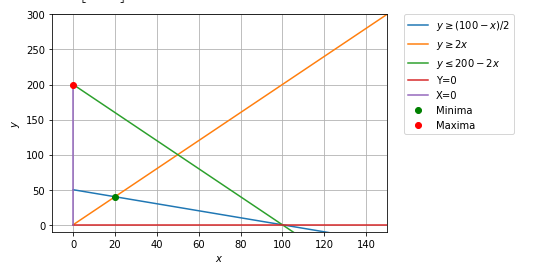
\includegraphics[width=\columnwidth]{./solutions/line_plane/46/plot.png}
%\label{figure 1}
%\end{figure}
